\begin{figure}[htbp]
  \centering
  \caption{Distribuição individual das 30 sementes frente à Melhor Solução Conhecida (MSC) nas instâncias 	exttt{B/0012} e 	exttt{B/0013}. Pontos representam as sementes individuais com dispersão vertical sutil (	extit{jitter}); losangos brancos indicam a média amostral; e a estrela escura sinaliza a Melhor Semente (	extbf{Nova MSC}). A zona sombreada em verde claro demarca a região de superação da MSC ($\Delta > 0$, $\mathrm{RPD} < 0\%$).}
  \label{fig:novas_msc_dotplot_sementes}
  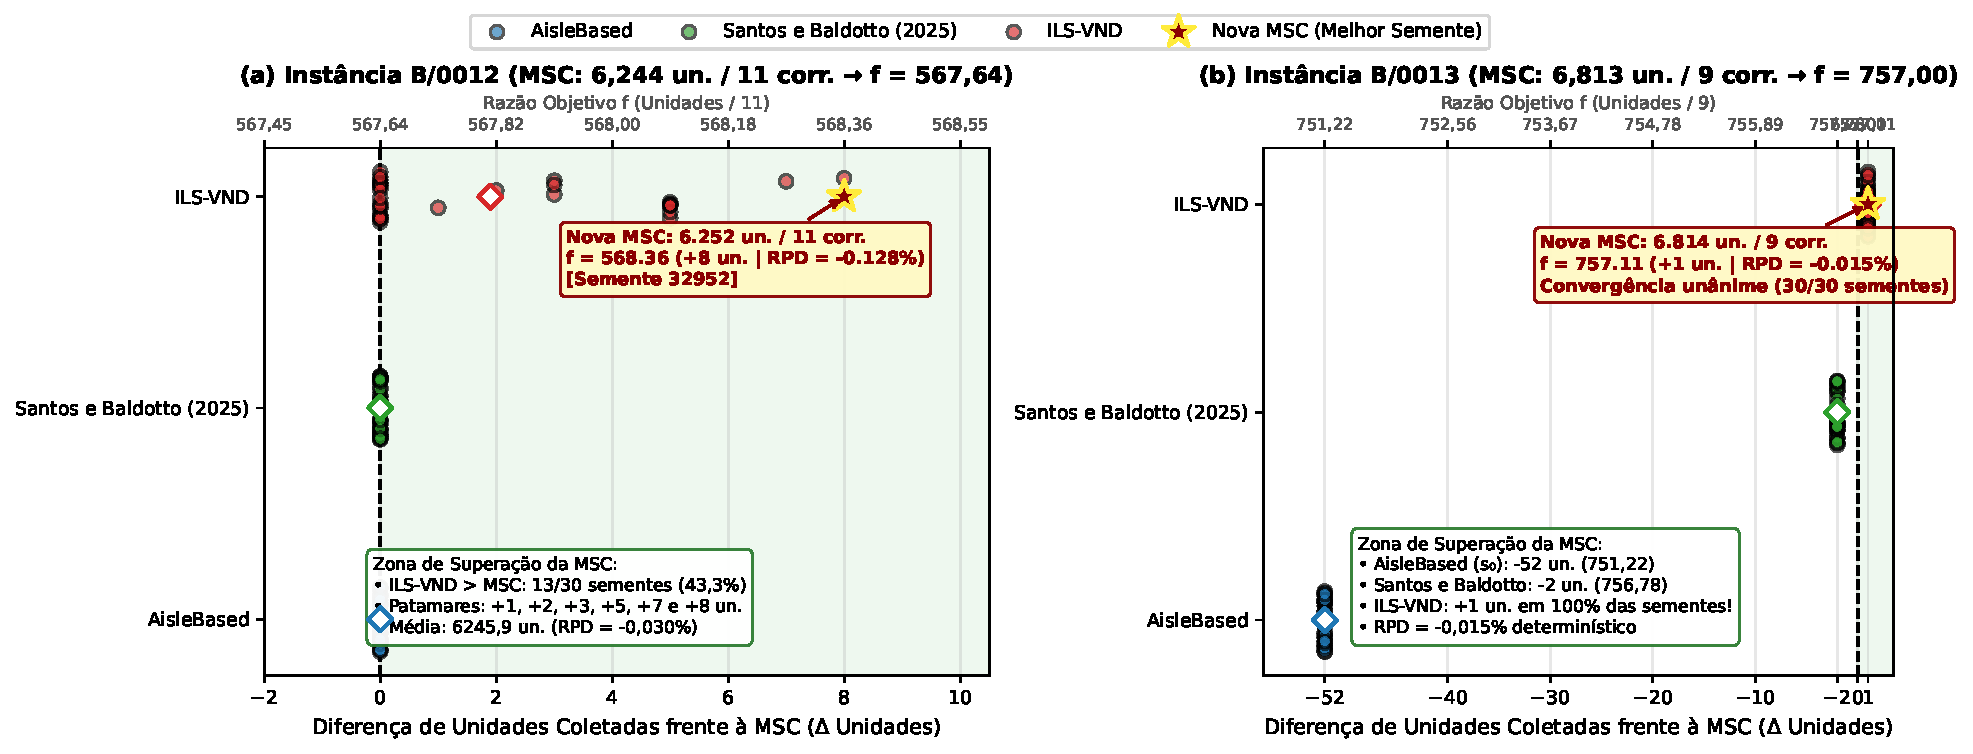
\includegraphics[width=0.98	extwidth]{img/novas_msc_dotplot_sementes.pdf}
  \caption*{\footnotesize Fonte: Elaborado pelo autor, 2026.}
\end{figure}
